
    




    
\documentclass[11pt]{article}

    
    \usepackage[breakable]{tcolorbox}
    \tcbset{nobeforeafter} % prevents tcolorboxes being placing in paragraphs
    \usepackage{float}
    \floatplacement{figure}{H} % forces figures to be placed at the correct location
    
    \usepackage[T1]{fontenc}
    % Nicer default font (+ math font) than Computer Modern for most use cases
    \usepackage{mathpazo}

    % Basic figure setup, for now with no caption control since it's done
    % automatically by Pandoc (which extracts ![](path) syntax from Markdown).
    \usepackage{graphicx}
    % We will generate all images so they have a width \maxwidth. This means
    % that they will get their normal width if they fit onto the page, but
    % are scaled down if they would overflow the margins.
    \makeatletter
    \def\maxwidth{\ifdim\Gin@nat@width>\linewidth\linewidth
    \else\Gin@nat@width\fi}
    \makeatother
    \let\Oldincludegraphics\includegraphics
    % Set max figure width to be 80% of text width, for now hardcoded.
    \renewcommand{\includegraphics}[1]{\Oldincludegraphics[width=.8\maxwidth]{#1}}
    % Ensure that by default, figures have no caption (until we provide a
    % proper Figure object with a Caption API and a way to capture that
    % in the conversion process - todo).
    \usepackage{caption}
    \DeclareCaptionLabelFormat{nolabel}{}
    \captionsetup{labelformat=nolabel}

    \usepackage{adjustbox} % Used to constrain images to a maximum size 
    \usepackage{xcolor} % Allow colors to be defined
    \usepackage{enumerate} % Needed for markdown enumerations to work
    \usepackage{geometry} % Used to adjust the document margins
    \usepackage{amsmath} % Equations
    \usepackage{amssymb} % Equations
    \usepackage{textcomp} % defines textquotesingle
    % Hack from http://tex.stackexchange.com/a/47451/13684:
    \AtBeginDocument{%
        \def\PYZsq{\textquotesingle}% Upright quotes in Pygmentized code
    }
    \usepackage{upquote} % Upright quotes for verbatim code
    \usepackage{eurosym} % defines \euro
    \usepackage[mathletters]{ucs} % Extended unicode (utf-8) support
    \usepackage[utf8x]{inputenc} % Allow utf-8 characters in the tex document
    \usepackage{fancyvrb} % verbatim replacement that allows latex
    \usepackage{grffile} % extends the file name processing of package graphics 
                         % to support a larger range 
    % The hyperref package gives us a pdf with properly built
    % internal navigation ('pdf bookmarks' for the table of contents,
    % internal cross-reference links, web links for URLs, etc.)
    \usepackage{hyperref}
    \usepackage{longtable} % longtable support required by pandoc >1.10
    \usepackage{booktabs}  % table support for pandoc > 1.12.2
    \usepackage[inline]{enumitem} % IRkernel/repr support (it uses the enumerate* environment)
    \usepackage[normalem]{ulem} % ulem is needed to support strikethroughs (\sout)
                                % normalem makes italics be italics, not underlines
    \usepackage{mathrsfs}
    

    
    % Colors for the hyperref package
    \definecolor{urlcolor}{rgb}{0,.145,.698}
    \definecolor{linkcolor}{rgb}{.71,0.21,0.01}
    \definecolor{citecolor}{rgb}{.12,.54,.11}

    % ANSI colors
    \definecolor{ansi-black}{HTML}{3E424D}
    \definecolor{ansi-black-intense}{HTML}{282C36}
    \definecolor{ansi-red}{HTML}{E75C58}
    \definecolor{ansi-red-intense}{HTML}{B22B31}
    \definecolor{ansi-green}{HTML}{00A250}
    \definecolor{ansi-green-intense}{HTML}{007427}
    \definecolor{ansi-yellow}{HTML}{DDB62B}
    \definecolor{ansi-yellow-intense}{HTML}{B27D12}
    \definecolor{ansi-blue}{HTML}{208FFB}
    \definecolor{ansi-blue-intense}{HTML}{0065CA}
    \definecolor{ansi-magenta}{HTML}{D160C4}
    \definecolor{ansi-magenta-intense}{HTML}{A03196}
    \definecolor{ansi-cyan}{HTML}{60C6C8}
    \definecolor{ansi-cyan-intense}{HTML}{258F8F}
    \definecolor{ansi-white}{HTML}{C5C1B4}
    \definecolor{ansi-white-intense}{HTML}{A1A6B2}
    \definecolor{ansi-default-inverse-fg}{HTML}{FFFFFF}
    \definecolor{ansi-default-inverse-bg}{HTML}{000000}

    % commands and environments needed by pandoc snippets
    % extracted from the output of `pandoc -s`
    \providecommand{\tightlist}{%
      \setlength{\itemsep}{0pt}\setlength{\parskip}{0pt}}
    \DefineVerbatimEnvironment{Highlighting}{Verbatim}{commandchars=\\\{\}}
    % Add ',fontsize=\small' for more characters per line
    \newenvironment{Shaded}{}{}
    \newcommand{\KeywordTok}[1]{\textcolor[rgb]{0.00,0.44,0.13}{\textbf{{#1}}}}
    \newcommand{\DataTypeTok}[1]{\textcolor[rgb]{0.56,0.13,0.00}{{#1}}}
    \newcommand{\DecValTok}[1]{\textcolor[rgb]{0.25,0.63,0.44}{{#1}}}
    \newcommand{\BaseNTok}[1]{\textcolor[rgb]{0.25,0.63,0.44}{{#1}}}
    \newcommand{\FloatTok}[1]{\textcolor[rgb]{0.25,0.63,0.44}{{#1}}}
    \newcommand{\CharTok}[1]{\textcolor[rgb]{0.25,0.44,0.63}{{#1}}}
    \newcommand{\StringTok}[1]{\textcolor[rgb]{0.25,0.44,0.63}{{#1}}}
    \newcommand{\CommentTok}[1]{\textcolor[rgb]{0.38,0.63,0.69}{\textit{{#1}}}}
    \newcommand{\OtherTok}[1]{\textcolor[rgb]{0.00,0.44,0.13}{{#1}}}
    \newcommand{\AlertTok}[1]{\textcolor[rgb]{1.00,0.00,0.00}{\textbf{{#1}}}}
    \newcommand{\FunctionTok}[1]{\textcolor[rgb]{0.02,0.16,0.49}{{#1}}}
    \newcommand{\RegionMarkerTok}[1]{{#1}}
    \newcommand{\ErrorTok}[1]{\textcolor[rgb]{1.00,0.00,0.00}{\textbf{{#1}}}}
    \newcommand{\NormalTok}[1]{{#1}}
    
    % Additional commands for more recent versions of Pandoc
    \newcommand{\ConstantTok}[1]{\textcolor[rgb]{0.53,0.00,0.00}{{#1}}}
    \newcommand{\SpecialCharTok}[1]{\textcolor[rgb]{0.25,0.44,0.63}{{#1}}}
    \newcommand{\VerbatimStringTok}[1]{\textcolor[rgb]{0.25,0.44,0.63}{{#1}}}
    \newcommand{\SpecialStringTok}[1]{\textcolor[rgb]{0.73,0.40,0.53}{{#1}}}
    \newcommand{\ImportTok}[1]{{#1}}
    \newcommand{\DocumentationTok}[1]{\textcolor[rgb]{0.73,0.13,0.13}{\textit{{#1}}}}
    \newcommand{\AnnotationTok}[1]{\textcolor[rgb]{0.38,0.63,0.69}{\textbf{\textit{{#1}}}}}
    \newcommand{\CommentVarTok}[1]{\textcolor[rgb]{0.38,0.63,0.69}{\textbf{\textit{{#1}}}}}
    \newcommand{\VariableTok}[1]{\textcolor[rgb]{0.10,0.09,0.49}{{#1}}}
    \newcommand{\ControlFlowTok}[1]{\textcolor[rgb]{0.00,0.44,0.13}{\textbf{{#1}}}}
    \newcommand{\OperatorTok}[1]{\textcolor[rgb]{0.40,0.40,0.40}{{#1}}}
    \newcommand{\BuiltInTok}[1]{{#1}}
    \newcommand{\ExtensionTok}[1]{{#1}}
    \newcommand{\PreprocessorTok}[1]{\textcolor[rgb]{0.74,0.48,0.00}{{#1}}}
    \newcommand{\AttributeTok}[1]{\textcolor[rgb]{0.49,0.56,0.16}{{#1}}}
    \newcommand{\InformationTok}[1]{\textcolor[rgb]{0.38,0.63,0.69}{\textbf{\textit{{#1}}}}}
    \newcommand{\WarningTok}[1]{\textcolor[rgb]{0.38,0.63,0.69}{\textbf{\textit{{#1}}}}}
    
    
    % Define a nice break command that doesn't care if a line doesn't already
    % exist.
    \def\br{\hspace*{\fill} \\* }
    % Math Jax compatibility definitions
    \def\gt{>}
    \def\lt{<}
    \let\Oldtex\TeX
    \let\Oldlatex\LaTeX
    \renewcommand{\TeX}{\textrm{\Oldtex}}
    \renewcommand{\LaTeX}{\textrm{\Oldlatex}}
    % Document parameters
    % Document title
    \title{Step1\_ConvexProgramming}
    
    
    
    
    
% Pygments definitions
\makeatletter
\def\PY@reset{\let\PY@it=\relax \let\PY@bf=\relax%
    \let\PY@ul=\relax \let\PY@tc=\relax%
    \let\PY@bc=\relax \let\PY@ff=\relax}
\def\PY@tok#1{\csname PY@tok@#1\endcsname}
\def\PY@toks#1+{\ifx\relax#1\empty\else%
    \PY@tok{#1}\expandafter\PY@toks\fi}
\def\PY@do#1{\PY@bc{\PY@tc{\PY@ul{%
    \PY@it{\PY@bf{\PY@ff{#1}}}}}}}
\def\PY#1#2{\PY@reset\PY@toks#1+\relax+\PY@do{#2}}

\expandafter\def\csname PY@tok@w\endcsname{\def\PY@tc##1{\textcolor[rgb]{0.73,0.73,0.73}{##1}}}
\expandafter\def\csname PY@tok@c\endcsname{\let\PY@it=\textit\def\PY@tc##1{\textcolor[rgb]{0.25,0.50,0.50}{##1}}}
\expandafter\def\csname PY@tok@cp\endcsname{\def\PY@tc##1{\textcolor[rgb]{0.74,0.48,0.00}{##1}}}
\expandafter\def\csname PY@tok@k\endcsname{\let\PY@bf=\textbf\def\PY@tc##1{\textcolor[rgb]{0.00,0.50,0.00}{##1}}}
\expandafter\def\csname PY@tok@kp\endcsname{\def\PY@tc##1{\textcolor[rgb]{0.00,0.50,0.00}{##1}}}
\expandafter\def\csname PY@tok@kt\endcsname{\def\PY@tc##1{\textcolor[rgb]{0.69,0.00,0.25}{##1}}}
\expandafter\def\csname PY@tok@o\endcsname{\def\PY@tc##1{\textcolor[rgb]{0.40,0.40,0.40}{##1}}}
\expandafter\def\csname PY@tok@ow\endcsname{\let\PY@bf=\textbf\def\PY@tc##1{\textcolor[rgb]{0.67,0.13,1.00}{##1}}}
\expandafter\def\csname PY@tok@nb\endcsname{\def\PY@tc##1{\textcolor[rgb]{0.00,0.50,0.00}{##1}}}
\expandafter\def\csname PY@tok@nf\endcsname{\def\PY@tc##1{\textcolor[rgb]{0.00,0.00,1.00}{##1}}}
\expandafter\def\csname PY@tok@nc\endcsname{\let\PY@bf=\textbf\def\PY@tc##1{\textcolor[rgb]{0.00,0.00,1.00}{##1}}}
\expandafter\def\csname PY@tok@nn\endcsname{\let\PY@bf=\textbf\def\PY@tc##1{\textcolor[rgb]{0.00,0.00,1.00}{##1}}}
\expandafter\def\csname PY@tok@ne\endcsname{\let\PY@bf=\textbf\def\PY@tc##1{\textcolor[rgb]{0.82,0.25,0.23}{##1}}}
\expandafter\def\csname PY@tok@nv\endcsname{\def\PY@tc##1{\textcolor[rgb]{0.10,0.09,0.49}{##1}}}
\expandafter\def\csname PY@tok@no\endcsname{\def\PY@tc##1{\textcolor[rgb]{0.53,0.00,0.00}{##1}}}
\expandafter\def\csname PY@tok@nl\endcsname{\def\PY@tc##1{\textcolor[rgb]{0.63,0.63,0.00}{##1}}}
\expandafter\def\csname PY@tok@ni\endcsname{\let\PY@bf=\textbf\def\PY@tc##1{\textcolor[rgb]{0.60,0.60,0.60}{##1}}}
\expandafter\def\csname PY@tok@na\endcsname{\def\PY@tc##1{\textcolor[rgb]{0.49,0.56,0.16}{##1}}}
\expandafter\def\csname PY@tok@nt\endcsname{\let\PY@bf=\textbf\def\PY@tc##1{\textcolor[rgb]{0.00,0.50,0.00}{##1}}}
\expandafter\def\csname PY@tok@nd\endcsname{\def\PY@tc##1{\textcolor[rgb]{0.67,0.13,1.00}{##1}}}
\expandafter\def\csname PY@tok@s\endcsname{\def\PY@tc##1{\textcolor[rgb]{0.73,0.13,0.13}{##1}}}
\expandafter\def\csname PY@tok@sd\endcsname{\let\PY@it=\textit\def\PY@tc##1{\textcolor[rgb]{0.73,0.13,0.13}{##1}}}
\expandafter\def\csname PY@tok@si\endcsname{\let\PY@bf=\textbf\def\PY@tc##1{\textcolor[rgb]{0.73,0.40,0.53}{##1}}}
\expandafter\def\csname PY@tok@se\endcsname{\let\PY@bf=\textbf\def\PY@tc##1{\textcolor[rgb]{0.73,0.40,0.13}{##1}}}
\expandafter\def\csname PY@tok@sr\endcsname{\def\PY@tc##1{\textcolor[rgb]{0.73,0.40,0.53}{##1}}}
\expandafter\def\csname PY@tok@ss\endcsname{\def\PY@tc##1{\textcolor[rgb]{0.10,0.09,0.49}{##1}}}
\expandafter\def\csname PY@tok@sx\endcsname{\def\PY@tc##1{\textcolor[rgb]{0.00,0.50,0.00}{##1}}}
\expandafter\def\csname PY@tok@m\endcsname{\def\PY@tc##1{\textcolor[rgb]{0.40,0.40,0.40}{##1}}}
\expandafter\def\csname PY@tok@gh\endcsname{\let\PY@bf=\textbf\def\PY@tc##1{\textcolor[rgb]{0.00,0.00,0.50}{##1}}}
\expandafter\def\csname PY@tok@gu\endcsname{\let\PY@bf=\textbf\def\PY@tc##1{\textcolor[rgb]{0.50,0.00,0.50}{##1}}}
\expandafter\def\csname PY@tok@gd\endcsname{\def\PY@tc##1{\textcolor[rgb]{0.63,0.00,0.00}{##1}}}
\expandafter\def\csname PY@tok@gi\endcsname{\def\PY@tc##1{\textcolor[rgb]{0.00,0.63,0.00}{##1}}}
\expandafter\def\csname PY@tok@gr\endcsname{\def\PY@tc##1{\textcolor[rgb]{1.00,0.00,0.00}{##1}}}
\expandafter\def\csname PY@tok@ge\endcsname{\let\PY@it=\textit}
\expandafter\def\csname PY@tok@gs\endcsname{\let\PY@bf=\textbf}
\expandafter\def\csname PY@tok@gp\endcsname{\let\PY@bf=\textbf\def\PY@tc##1{\textcolor[rgb]{0.00,0.00,0.50}{##1}}}
\expandafter\def\csname PY@tok@go\endcsname{\def\PY@tc##1{\textcolor[rgb]{0.53,0.53,0.53}{##1}}}
\expandafter\def\csname PY@tok@gt\endcsname{\def\PY@tc##1{\textcolor[rgb]{0.00,0.27,0.87}{##1}}}
\expandafter\def\csname PY@tok@err\endcsname{\def\PY@bc##1{\setlength{\fboxsep}{0pt}\fcolorbox[rgb]{1.00,0.00,0.00}{1,1,1}{\strut ##1}}}
\expandafter\def\csname PY@tok@kc\endcsname{\let\PY@bf=\textbf\def\PY@tc##1{\textcolor[rgb]{0.00,0.50,0.00}{##1}}}
\expandafter\def\csname PY@tok@kd\endcsname{\let\PY@bf=\textbf\def\PY@tc##1{\textcolor[rgb]{0.00,0.50,0.00}{##1}}}
\expandafter\def\csname PY@tok@kn\endcsname{\let\PY@bf=\textbf\def\PY@tc##1{\textcolor[rgb]{0.00,0.50,0.00}{##1}}}
\expandafter\def\csname PY@tok@kr\endcsname{\let\PY@bf=\textbf\def\PY@tc##1{\textcolor[rgb]{0.00,0.50,0.00}{##1}}}
\expandafter\def\csname PY@tok@bp\endcsname{\def\PY@tc##1{\textcolor[rgb]{0.00,0.50,0.00}{##1}}}
\expandafter\def\csname PY@tok@fm\endcsname{\def\PY@tc##1{\textcolor[rgb]{0.00,0.00,1.00}{##1}}}
\expandafter\def\csname PY@tok@vc\endcsname{\def\PY@tc##1{\textcolor[rgb]{0.10,0.09,0.49}{##1}}}
\expandafter\def\csname PY@tok@vg\endcsname{\def\PY@tc##1{\textcolor[rgb]{0.10,0.09,0.49}{##1}}}
\expandafter\def\csname PY@tok@vi\endcsname{\def\PY@tc##1{\textcolor[rgb]{0.10,0.09,0.49}{##1}}}
\expandafter\def\csname PY@tok@vm\endcsname{\def\PY@tc##1{\textcolor[rgb]{0.10,0.09,0.49}{##1}}}
\expandafter\def\csname PY@tok@sa\endcsname{\def\PY@tc##1{\textcolor[rgb]{0.73,0.13,0.13}{##1}}}
\expandafter\def\csname PY@tok@sb\endcsname{\def\PY@tc##1{\textcolor[rgb]{0.73,0.13,0.13}{##1}}}
\expandafter\def\csname PY@tok@sc\endcsname{\def\PY@tc##1{\textcolor[rgb]{0.73,0.13,0.13}{##1}}}
\expandafter\def\csname PY@tok@dl\endcsname{\def\PY@tc##1{\textcolor[rgb]{0.73,0.13,0.13}{##1}}}
\expandafter\def\csname PY@tok@s2\endcsname{\def\PY@tc##1{\textcolor[rgb]{0.73,0.13,0.13}{##1}}}
\expandafter\def\csname PY@tok@sh\endcsname{\def\PY@tc##1{\textcolor[rgb]{0.73,0.13,0.13}{##1}}}
\expandafter\def\csname PY@tok@s1\endcsname{\def\PY@tc##1{\textcolor[rgb]{0.73,0.13,0.13}{##1}}}
\expandafter\def\csname PY@tok@mb\endcsname{\def\PY@tc##1{\textcolor[rgb]{0.40,0.40,0.40}{##1}}}
\expandafter\def\csname PY@tok@mf\endcsname{\def\PY@tc##1{\textcolor[rgb]{0.40,0.40,0.40}{##1}}}
\expandafter\def\csname PY@tok@mh\endcsname{\def\PY@tc##1{\textcolor[rgb]{0.40,0.40,0.40}{##1}}}
\expandafter\def\csname PY@tok@mi\endcsname{\def\PY@tc##1{\textcolor[rgb]{0.40,0.40,0.40}{##1}}}
\expandafter\def\csname PY@tok@il\endcsname{\def\PY@tc##1{\textcolor[rgb]{0.40,0.40,0.40}{##1}}}
\expandafter\def\csname PY@tok@mo\endcsname{\def\PY@tc##1{\textcolor[rgb]{0.40,0.40,0.40}{##1}}}
\expandafter\def\csname PY@tok@ch\endcsname{\let\PY@it=\textit\def\PY@tc##1{\textcolor[rgb]{0.25,0.50,0.50}{##1}}}
\expandafter\def\csname PY@tok@cm\endcsname{\let\PY@it=\textit\def\PY@tc##1{\textcolor[rgb]{0.25,0.50,0.50}{##1}}}
\expandafter\def\csname PY@tok@cpf\endcsname{\let\PY@it=\textit\def\PY@tc##1{\textcolor[rgb]{0.25,0.50,0.50}{##1}}}
\expandafter\def\csname PY@tok@c1\endcsname{\let\PY@it=\textit\def\PY@tc##1{\textcolor[rgb]{0.25,0.50,0.50}{##1}}}
\expandafter\def\csname PY@tok@cs\endcsname{\let\PY@it=\textit\def\PY@tc##1{\textcolor[rgb]{0.25,0.50,0.50}{##1}}}

\def\PYZbs{\char`\\}
\def\PYZus{\char`\_}
\def\PYZob{\char`\{}
\def\PYZcb{\char`\}}
\def\PYZca{\char`\^}
\def\PYZam{\char`\&}
\def\PYZlt{\char`\<}
\def\PYZgt{\char`\>}
\def\PYZsh{\char`\#}
\def\PYZpc{\char`\%}
\def\PYZdl{\char`\$}
\def\PYZhy{\char`\-}
\def\PYZsq{\char`\'}
\def\PYZdq{\char`\"}
\def\PYZti{\char`\~}
% for compatibility with earlier versions
\def\PYZat{@}
\def\PYZlb{[}
\def\PYZrb{]}
\makeatother


    % For linebreaks inside Verbatim environment from package fancyvrb. 
    \makeatletter
        \newbox\Wrappedcontinuationbox 
        \newbox\Wrappedvisiblespacebox 
        \newcommand*\Wrappedvisiblespace {\textcolor{red}{\textvisiblespace}} 
        \newcommand*\Wrappedcontinuationsymbol {\textcolor{red}{\llap{\tiny$\m@th\hookrightarrow$}}} 
        \newcommand*\Wrappedcontinuationindent {3ex } 
        \newcommand*\Wrappedafterbreak {\kern\Wrappedcontinuationindent\copy\Wrappedcontinuationbox} 
        % Take advantage of the already applied Pygments mark-up to insert 
        % potential linebreaks for TeX processing. 
        %        {, <, #, %, $, ' and ": go to next line. 
        %        _, }, ^, &, >, - and ~: stay at end of broken line. 
        % Use of \textquotesingle for straight quote. 
        \newcommand*\Wrappedbreaksatspecials {% 
            \def\PYGZus{\discretionary{\char`\_}{\Wrappedafterbreak}{\char`\_}}% 
            \def\PYGZob{\discretionary{}{\Wrappedafterbreak\char`\{}{\char`\{}}% 
            \def\PYGZcb{\discretionary{\char`\}}{\Wrappedafterbreak}{\char`\}}}% 
            \def\PYGZca{\discretionary{\char`\^}{\Wrappedafterbreak}{\char`\^}}% 
            \def\PYGZam{\discretionary{\char`\&}{\Wrappedafterbreak}{\char`\&}}% 
            \def\PYGZlt{\discretionary{}{\Wrappedafterbreak\char`\<}{\char`\<}}% 
            \def\PYGZgt{\discretionary{\char`\>}{\Wrappedafterbreak}{\char`\>}}% 
            \def\PYGZsh{\discretionary{}{\Wrappedafterbreak\char`\#}{\char`\#}}% 
            \def\PYGZpc{\discretionary{}{\Wrappedafterbreak\char`\%}{\char`\%}}% 
            \def\PYGZdl{\discretionary{}{\Wrappedafterbreak\char`\$}{\char`\$}}% 
            \def\PYGZhy{\discretionary{\char`\-}{\Wrappedafterbreak}{\char`\-}}% 
            \def\PYGZsq{\discretionary{}{\Wrappedafterbreak\textquotesingle}{\textquotesingle}}% 
            \def\PYGZdq{\discretionary{}{\Wrappedafterbreak\char`\"}{\char`\"}}% 
            \def\PYGZti{\discretionary{\char`\~}{\Wrappedafterbreak}{\char`\~}}% 
        } 
        % Some characters . , ; ? ! / are not pygmentized. 
        % This macro makes them "active" and they will insert potential linebreaks 
        \newcommand*\Wrappedbreaksatpunct {% 
            \lccode`\~`\.\lowercase{\def~}{\discretionary{\hbox{\char`\.}}{\Wrappedafterbreak}{\hbox{\char`\.}}}% 
            \lccode`\~`\,\lowercase{\def~}{\discretionary{\hbox{\char`\,}}{\Wrappedafterbreak}{\hbox{\char`\,}}}% 
            \lccode`\~`\;\lowercase{\def~}{\discretionary{\hbox{\char`\;}}{\Wrappedafterbreak}{\hbox{\char`\;}}}% 
            \lccode`\~`\:\lowercase{\def~}{\discretionary{\hbox{\char`\:}}{\Wrappedafterbreak}{\hbox{\char`\:}}}% 
            \lccode`\~`\?\lowercase{\def~}{\discretionary{\hbox{\char`\?}}{\Wrappedafterbreak}{\hbox{\char`\?}}}% 
            \lccode`\~`\!\lowercase{\def~}{\discretionary{\hbox{\char`\!}}{\Wrappedafterbreak}{\hbox{\char`\!}}}% 
            \lccode`\~`\/\lowercase{\def~}{\discretionary{\hbox{\char`\/}}{\Wrappedafterbreak}{\hbox{\char`\/}}}% 
            \catcode`\.\active
            \catcode`\,\active 
            \catcode`\;\active
            \catcode`\:\active
            \catcode`\?\active
            \catcode`\!\active
            \catcode`\/\active 
            \lccode`\~`\~ 	
        }
    \makeatother

    \let\OriginalVerbatim=\Verbatim
    \makeatletter
    \renewcommand{\Verbatim}[1][1]{%
        %\parskip\z@skip
        \sbox\Wrappedcontinuationbox {\Wrappedcontinuationsymbol}%
        \sbox\Wrappedvisiblespacebox {\FV@SetupFont\Wrappedvisiblespace}%
        \def\FancyVerbFormatLine ##1{\hsize\linewidth
            \vtop{\raggedright\hyphenpenalty\z@\exhyphenpenalty\z@
                \doublehyphendemerits\z@\finalhyphendemerits\z@
                \strut ##1\strut}%
        }%
        % If the linebreak is at a space, the latter will be displayed as visible
        % space at end of first line, and a continuation symbol starts next line.
        % Stretch/shrink are however usually zero for typewriter font.
        \def\FV@Space {%
            \nobreak\hskip\z@ plus\fontdimen3\font minus\fontdimen4\font
            \discretionary{\copy\Wrappedvisiblespacebox}{\Wrappedafterbreak}
            {\kern\fontdimen2\font}%
        }%
        
        % Allow breaks at special characters using \PYG... macros.
        \Wrappedbreaksatspecials
        % Breaks at punctuation characters . , ; ? ! and / need catcode=\active 	
        \OriginalVerbatim[#1,codes*=\Wrappedbreaksatpunct]%
    }
    \makeatother

    % Exact colors from NB
    \definecolor{incolor}{HTML}{303F9F}
    \definecolor{outcolor}{HTML}{D84315}
    \definecolor{cellborder}{HTML}{CFCFCF}
    \definecolor{cellbackground}{HTML}{F7F7F7}
    
    % prompt
    \newcommand{\prompt}[4]{
        \llap{{\color{#2}[#3]: #4}}\vspace{-1.25em}
    }
    

    
    % Prevent overflowing lines due to hard-to-break entities
    \sloppy 
    % Setup hyperref package
    \hypersetup{
      breaklinks=true,  % so long urls are correctly broken across lines
      colorlinks=true,
      urlcolor=urlcolor,
      linkcolor=linkcolor,
      citecolor=citecolor,
      }
    % Slightly bigger margins than the latex defaults
    
    \geometry{verbose,tmargin=1in,bmargin=1in,lmargin=1in,rmargin=1in}
    
    

    \begin{document}
    
    
    \maketitle
    
    

    
    \begin{tcolorbox}[breakable, size=fbox, boxrule=1pt, pad at break*=1mm,colback=cellbackground, colframe=cellborder]
\prompt{In}{incolor}{ }{\hspace{4pt}}
\begin{Verbatim}[commandchars=\\\{\}]
\PY{k}{using} \PY{n}{Convex}
\PY{k}{using} \PY{n}{GLPK}
\PY{k}{using} \PY{n}{Printf}
\end{Verbatim}
\end{tcolorbox}

    \section{Introduction to convex
optimization}\label{introduction-to-convex-optimization}

\begin{equation}
\label{Eq:Program}
  \begin{array}{rll}
    \text{minimize} & f (\vec{x}) & \\
    \text{over} & \vec{x} \in R^n & \\
    & g_j (\vec{x}) \leq 0 & j \in \mathcal{J}\\
    & h_k (\vec{x}) = 0 & k \in \mathcal{K}
  \end{array}
\end{equation}

where all \(f\), \(g_j\) and \(h_k\) are convex; for \(f(\vec{x})\):

\begin{equation}
  \label{Eq:Convex}
  f (\alpha \vec{x}_1 + (1 - \alpha) \vec{x}_2) \leqslant  \alpha f (\vec{x}_1) + (1 - \alpha) f (\vec{x}_2), \qquad \alpha \in [0, 1]
\end{equation}

On left, an example of a convex function is given below, where we plot
the line segment
\(\color{blue}{\alpha f (\vec{x}_1) + (1 - \alpha) f (\vec{x}_2)}\) in
dark blue. On the right, an example of a nonconvex function.

\begin{figure}
\centering
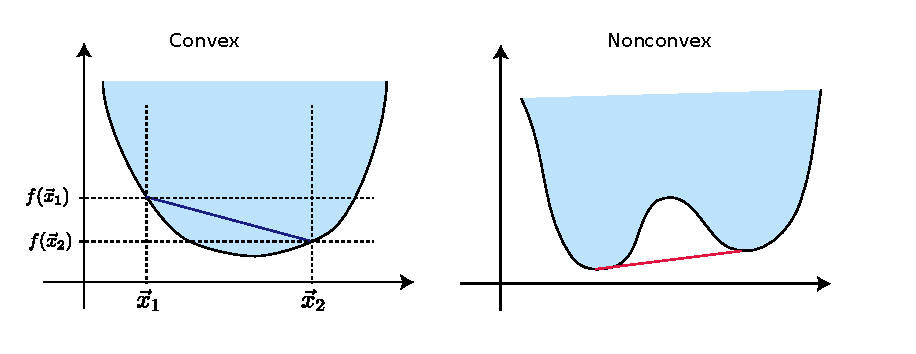
\includegraphics{ConvexFun.pdf}
\caption{ConvexFun.svg}
\end{figure}

In the same spirit, convex sets include the line segment between any two
of their points:

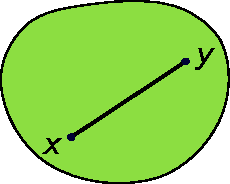
\includegraphics{Convex_polygon_illustration1.pdf}

while convex sets do not:

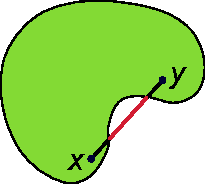
\includegraphics{Convex_polygon_illustration2.pdf}

Convex programs \eqref{Eq:Program} have one crucial property: any local
minimum is also a global minimum. In particular, this guarantees that
(non pathological) optimization algorithms always find the global
minimum up to numerical precision.

\subsection{Linear optimization}\label{linear-optimization}

The simplest kind of convex programs is a \emph{linear program}, where
the objective and all constraints are represented by linear functions
such as (technically, these are \emph{affine functions}):

\begin{equation}
f(\vec{x}) = \vec{c}^\top \vec{x} + d
\end{equation}

\begin{equation}
\label{Eq:LPExample}
  \begin{array}{rl}
    p^\star = \text{minimize} & x_1 + 2 x_2 - x_3 \\
    \text{over} & \vec{x} \in R^3 \\
    & x_1, x_2, x_3 \ge 0 \\
    & x_1 + x_2 + x_3 = 1
  \end{array}
\end{equation}

We now solve that problem using the
\href{https://github.com/JuliaOpt/Convex.jl}{Convex.jl} optimization
toolbox.

    \begin{tcolorbox}[breakable, size=fbox, boxrule=1pt, pad at break*=1mm,colback=cellbackground, colframe=cellborder]
\prompt{In}{incolor}{ }{\hspace{4pt}}
\begin{Verbatim}[commandchars=\\\{\}]
\PY{n}{x} \PY{o}{=} \PY{n}{Variable}\PY{p}{(}\PY{l+m+mi}{3}\PY{p}{)}
\PY{n}{constraints} \PY{o}{=} \PY{p}{[}\PY{n}{x} \PY{o}{\PYZgt{}=} \PY{l+m+mi}{0}\PY{p}{,} \PY{n}{sum}\PY{p}{(}\PY{n}{x}\PY{p}{)} \PY{o}{==} \PY{l+m+mi}{1}\PY{p}{]}
\PY{n}{objective} \PY{o}{=} \PY{n}{x}\PY{p}{[}\PY{l+m+mi}{1}\PY{p}{]} \PY{o}{+} \PY{l+m+mi}{2}\PY{o}{*}\PY{n}{x}\PY{p}{[}\PY{l+m+mi}{2}\PY{p}{]} \PY{o}{\PYZhy{}} \PY{n}{x}\PY{p}{[}\PY{l+m+mi}{3}\PY{p}{]}
\PY{n}{problem} \PY{o}{=} \PY{n}{Convex}\PY{o}{.}\PY{n}{minimize}\PY{p}{(}\PY{n}{objective}\PY{p}{,} \PY{n}{constraints}\PY{p}{)}
\PY{n}{solve!}\PY{p}{(}\PY{n}{problem}\PY{p}{,} \PY{n}{GLPK}\PY{o}{.}\PY{n}{Optimizer}\PY{p}{(}\PY{n}{msg\PYZus{}lev}\PY{o}{=}\PY{n}{GLPK}\PY{o}{.}\PY{n}{MSG\PYZus{}ALL} \PY{p}{)}\PY{p}{)}
\PY{n+nd}{@printf}\PY{p}{(}\PY{l+s}{\PYZdq{}}\PY{l+s+se}{\PYZbs{}n}\PY{l+s}{\PYZdq{}}\PY{p}{)}
\PY{n+nd}{@printf}\PY{p}{(}\PY{l+s}{\PYZdq{}}\PY{l+s}{O}\PY{l+s}{p}\PY{l+s}{t}\PY{l+s}{i}\PY{l+s}{m}\PY{l+s}{a}\PY{l+s}{l}\PY{l+s}{ }\PY{l+s}{o}\PY{l+s}{b}\PY{l+s}{j}\PY{l+s}{e}\PY{l+s}{c}\PY{l+s}{t}\PY{l+s}{i}\PY{l+s}{v}\PY{l+s}{e}\PY{l+s}{ }\PY{l+s}{p}\PY{l+s}{ }\PY{l+s}{=}\PY{l+s}{ }\PY{l+s+si}{\PYZpc{}f}\PY{l+s+se}{\PYZbs{}n}\PY{l+s}{\PYZdq{}}\PY{p}{,} \PY{n}{problem}\PY{o}{.}\PY{n}{optval}\PY{p}{)}
\PY{n+nd}{@printf}\PY{p}{(}\PY{l+s}{\PYZdq{}}\PY{l+s}{O}\PY{l+s}{p}\PY{l+s}{t}\PY{l+s}{i}\PY{l+s}{m}\PY{l+s}{a}\PY{l+s}{l}\PY{l+s}{ }\PY{l+s}{p}\PY{l+s}{o}\PY{l+s}{i}\PY{l+s}{n}\PY{l+s}{t}\PY{l+s}{ }\PY{l+s}{ }\PY{l+s}{ }\PY{l+s}{ }\PY{l+s}{ }\PY{l+s}{x}\PY{l+s}{ }\PY{l+s}{=}\PY{l+s}{ }\PY{l+s+si}{\PYZpc{}s}\PY{l+s+se}{\PYZbs{}n}\PY{l+s}{\PYZdq{}}\PY{p}{,} \PY{n}{x}\PY{o}{.}\PY{n}{value}\PY{p}{)}
\end{Verbatim}
\end{tcolorbox}

    \subsubsection{Primal canonical form of a linear
program}\label{primal-canonical-form-of-a-linear-program}

The standard form of a linear program is as follows, with
\(\vec{c} \in \mathbb{R}^n\), \(A \in \mathbb{R}^{m \times n}\) and
\(\vec{b} \in \mathbb{R}^m\).

\begin{equation}
\label{Eq:PrimalForm}
  \begin{array}{rl}
    \text{minimize} & \vec{c}^\top \vec{x} \\
    \text{over} & \vec{x} \in R^n \\
    & A \vec{x} = \vec{b} \\
    & \vec{x} \ge 0
  \end{array}
\end{equation}

The problem is fully specified by the matrix \(A\) and the vectors
\(\vec{b}\) and \(\vec{c}\).

\paragraph{Lecture exercice}\label{lecture-exercice}

Complete the program data below to solve \eqref{Eq:LPExample}.

    \begin{tcolorbox}[breakable, size=fbox, boxrule=1pt, pad at break*=1mm,colback=cellbackground, colframe=cellborder]
\prompt{In}{incolor}{ }{\hspace{4pt}}
\begin{Verbatim}[commandchars=\\\{\}]
\PY{k}{using} \PY{n}{Convex}
\PY{k}{using} \PY{n}{GLPK}
\PY{c}{\PYZsh{} remember [1, 1, 1] is a 1D vector, [1; 1; 1] is a column matrix, [1 1 1] is a row matrix}
\PY{n}{x} \PY{o}{=} \PY{n}{Variable}\PY{p}{(}\PY{l+m+mi}{3}\PY{p}{)}
\PY{n}{c} \PY{o}{=} \PY{p}{[}\PY{p}{]}
\PY{n}{A} \PY{o}{=} \PY{p}{[}\PY{p}{]}
\PY{n}{b} \PY{o}{=} \PY{p}{[}\PY{p}{]}
\PY{n}{constraints} \PY{o}{=} \PY{p}{[}\PY{n}{A}\PY{o}{*}\PY{n}{x} \PY{o}{==} \PY{n}{b}\PY{p}{,} \PY{n}{x} \PY{o}{\PYZgt{}=} \PY{l+m+mi}{0}\PY{p}{]}
\PY{n}{objective} \PY{o}{=} \PY{n}{dot}\PY{p}{(}\PY{n}{c}\PY{p}{,} \PY{n}{x}\PY{p}{)}
\PY{n}{problem} \PY{o}{=} \PY{n}{Convex}\PY{o}{.}\PY{n}{minimize}\PY{p}{(}\PY{n}{objective}\PY{p}{,} \PY{n}{constraints}\PY{p}{)}
\PY{n}{solve!}\PY{p}{(}\PY{n}{problem}\PY{p}{,} \PY{n}{GLPK}\PY{o}{.}\PY{n}{Optimizer}\PY{p}{(}\PY{n}{msg\PYZus{}lev}\PY{o}{=}\PY{n}{GLPK}\PY{o}{.}\PY{n}{MSG\PYZus{}ALL}\PY{p}{)}\PY{p}{)}
\PY{n+nd}{@printf}\PY{p}{(}\PY{l+s}{\PYZdq{}}\PY{l+s+se}{\PYZbs{}n}\PY{l+s}{\PYZdq{}}\PY{p}{)}
\PY{n+nd}{@printf}\PY{p}{(}\PY{l+s}{\PYZdq{}}\PY{l+s}{O}\PY{l+s}{p}\PY{l+s}{t}\PY{l+s}{i}\PY{l+s}{m}\PY{l+s}{a}\PY{l+s}{l}\PY{l+s}{ }\PY{l+s}{o}\PY{l+s}{b}\PY{l+s}{j}\PY{l+s}{e}\PY{l+s}{c}\PY{l+s}{t}\PY{l+s}{i}\PY{l+s}{v}\PY{l+s}{e}\PY{l+s}{ }\PY{l+s}{p}\PY{l+s}{ }\PY{l+s}{=}\PY{l+s}{ }\PY{l+s+si}{\PYZpc{}f}\PY{l+s+se}{\PYZbs{}n}\PY{l+s}{\PYZdq{}}\PY{p}{,} \PY{n}{problem}\PY{o}{.}\PY{n}{optval}\PY{p}{)}
\PY{n+nd}{@printf}\PY{p}{(}\PY{l+s}{\PYZdq{}}\PY{l+s}{O}\PY{l+s}{p}\PY{l+s}{t}\PY{l+s}{i}\PY{l+s}{m}\PY{l+s}{a}\PY{l+s}{l}\PY{l+s}{ }\PY{l+s}{p}\PY{l+s}{o}\PY{l+s}{i}\PY{l+s}{n}\PY{l+s}{t}\PY{l+s}{ }\PY{l+s}{ }\PY{l+s}{ }\PY{l+s}{ }\PY{l+s}{ }\PY{l+s}{x}\PY{l+s}{ }\PY{l+s}{=}\PY{l+s}{ }\PY{l+s+si}{\PYZpc{}s}\PY{l+s+se}{\PYZbs{}n}\PY{l+s}{\PYZdq{}}\PY{p}{,} \PY{n}{x}\PY{o}{.}\PY{n}{value}\PY{p}{)}
\end{Verbatim}
\end{tcolorbox}

    \subsection{Duality}\label{duality}

We remind the primal canonical form \eqref{Eq:PrimalForm}:

\begin{equation*}
  p^\star = \underset{\vec{x} \in R^n }{\text{minimize}} \quad \vec{c}^\top \vec{x}, \qquad A \vec{x} = \vec{b}, \qquad \vec{x} \ge 0,
\end{equation*}

and introduce the notation

\begin{itemize}
\tightlist
\item
  a variable with a \(\star\) superscript is an optimal solution (as in
  \(p^\star\) is the minimum of the LP),
\item
  a variable with a \(*\) superscript is a feasible solution (as in
  \(\vec{x}^*\) satisfies the constraints),
\end{itemize}

with the conventions

\begin{itemize}
\tightlist
\item
  \(p^\star = + \infty\) if the problem is infeasible,
\item
  \(p^\star\) is finite if the problem has an optimal (thus feasible)
  solution,
\item
  \(p^\star = -\infty\) if the problem is unbounded, as there are
  feasible solutions with \(\vec{c}^\top \vec{x} \rightarrow -\infty\).
\end{itemize}

We introduce the Lagrange multipliers \(\vec{y} \in \mathbb{R}^m\)
corresponding to the constraint \(A \vec{x} = \vec{b}\), and the
Lagrange multipliers \(\vec{s} \in \mathbb{R}^n\) corresponding to the
constraint \(\vec{x} \ge 0\), with \(\vec{s} \ge 0\) as they correspond
to an inequality constraint. The Lagrangian function is:

\begin{equation}
\label{Eq:Lagrangian}
L(\vec{x},\vec{y},\vec{s}) = \vec{c}^\top x + \vec{y}^\top (\vec{b} - A \vec{x}) - \vec{s}^\top \vec{x}.
\end{equation}

For any feasible \(\vec{x}^*\) and any \((\vec{y}^*, \vec{s}^*)\) with
\(\vec{s} \ge 0\), we have

\begin{equation}
\label{Eq:LowerBound}
L(\vec{x}^*,\vec{y}^*,\vec{s}^*) = \vec{c}^\top x^* + (\vec{y}^*)^\top \underbrace{(\vec{b} - A \vec{x}^*)}_{=0} - (\vec{s}^*)^\top \vec{x}^* \le \vec{c}^\top \vec{x}^*
\end{equation}

Let us now minimize \(L(\vec{x}, \vec{y}, \vec{s})\) over \(\vec{x}\):

\begin{equation}
\label{Eq:DualCases}
g(\vec{y}, \vec{s}) = \min_{\vec{x}} \vec{x}^\top (\vec{c} - A^\top \vec{y} - \vec{s}) + \vec{b}^\top \vec{y} = \begin{cases} \vec{b}^\top \vec{y}, & \vec{c} - A^\top \vec{y} - \vec{s} = 0, \\ -\infty, & \text{otherwise}. \end{cases}
\end{equation}

Note that for every \((\vec{y}, \vec{s})\) (with \(\vec{s} \ge 0\) by
definition), the value \(g(\vec{y}, \vec{s})\) is a lower bound for
\(p^\star\) by \eqref{Eq:LowerBound}.

In \eqref{Eq:DualCases}, only the first case
(\(\vec{c} - A^\top \vec{y} - \vec{s} = 0\)) leads to a nontrivial upper
bound. We now maximize over such \((\vec{y}, \vec{s})\) to get the best
lower bound.

\subsubsection{Dual canonical form of a linear
program}\label{dual-canonical-form-of-a-linear-program}

We obtain:

\begin{equation}
\label{Eq:DualForm}
  \begin{array}{rl}
    d^\star = \text{maximize} & \vec{b}^\top \vec{y} \\
    \text{over} & \vec{y} \in \mathbb{R}^m, \vec{s} \in \mathbb{S}^n \\
    & \vec{c} - A^\top \vec{y} = \vec{s} \\
    & \vec{s} \ge 0
  \end{array}
\end{equation}

which is the dual problem. Through the Lagrangian mechanism, we have
\(d^\star \le p^\star\) which is \emph{weak duality}.

We have the cases, for the dual problem: - \(d^\star = +\infty\), dual
unbounded, thus \(+\infty \le p^\star\) and the primal problem is
infeasible, - \(d^\star\) is finite, the dual is feasible, the primal
problem can either be feasible or infeasible (but not unbounded), -
\(d^\star = -\infty\), the dual problem is infeasible.

For linear programs only, when \(d^\star\) is finite, then
\(p^\star = d^\star\); when \(p^\star\) is finite, also
\(d^\star = p^\star\) (this is called \emph{strong duality}).

\paragraph{Lecture exercice}\label{lecture-exercice}

Fill the problem data below to solve the dual of \eqref{Eq:LPExample}.

    \begin{tcolorbox}[breakable, size=fbox, boxrule=1pt, pad at break*=1mm,colback=cellbackground, colframe=cellborder]
\prompt{In}{incolor}{ }{\hspace{4pt}}
\begin{Verbatim}[commandchars=\\\{\}]
\PY{k}{using} \PY{n}{Convex}
\PY{k}{using} \PY{n}{GLPK}
\PY{n}{y} \PY{o}{=} \PY{n}{Variable}\PY{p}{(}\PY{l+m+mi}{1}\PY{p}{)}
\PY{n}{s} \PY{o}{=} \PY{n}{Variable}\PY{p}{(}\PY{l+m+mi}{3}\PY{p}{)}
\PY{n}{c} \PY{o}{=} \PY{p}{[}\PY{p}{]}
\PY{n}{A} \PY{o}{=} \PY{p}{[}\PY{p}{]}
\PY{n}{b} \PY{o}{=} \PY{p}{[}\PY{p}{]}
\PY{n}{constraints} \PY{o}{=} \PY{p}{[}\PY{n}{s} \PY{o}{\PYZgt{}=} \PY{l+m+mi}{0}\PY{p}{,} \PY{n}{s} \PY{o}{==} \PY{n}{c} \PY{o}{\PYZhy{}} \PY{n}{transpose}\PY{p}{(}\PY{n}{A}\PY{p}{)}\PY{o}{*}\PY{n}{y}\PY{p}{]}
\PY{n}{objective} \PY{o}{=} \PY{n}{dot}\PY{p}{(}\PY{n}{b}\PY{p}{,} \PY{n}{y}\PY{p}{)}
\PY{n}{problem} \PY{o}{=} \PY{n}{Convex}\PY{o}{.}\PY{n}{maximize}\PY{p}{(}\PY{n}{objective}\PY{p}{,} \PY{n}{constraints}\PY{p}{)}
\PY{n}{solve!}\PY{p}{(}\PY{n}{problem}\PY{p}{,} \PY{n}{GLPK}\PY{o}{.}\PY{n}{Optimizer}\PY{p}{(}\PY{n}{msg\PYZus{}lev}\PY{o}{=}\PY{n}{GLPK}\PY{o}{.}\PY{n}{MSG\PYZus{}ALL}\PY{p}{)}\PY{p}{)}
\PY{n+nd}{@printf}\PY{p}{(}\PY{l+s}{\PYZdq{}}\PY{l+s+se}{\PYZbs{}n}\PY{l+s}{\PYZdq{}}\PY{p}{)}
\PY{n+nd}{@printf}\PY{p}{(}\PY{l+s}{\PYZdq{}}\PY{l+s}{O}\PY{l+s}{p}\PY{l+s}{t}\PY{l+s}{i}\PY{l+s}{m}\PY{l+s}{a}\PY{l+s}{l}\PY{l+s}{ }\PY{l+s}{o}\PY{l+s}{b}\PY{l+s}{j}\PY{l+s}{e}\PY{l+s}{c}\PY{l+s}{t}\PY{l+s}{i}\PY{l+s}{v}\PY{l+s}{e}\PY{l+s}{ }\PY{l+s}{d}\PY{l+s}{ }\PY{l+s}{=}\PY{l+s}{ }\PY{l+s+si}{\PYZpc{}f}\PY{l+s+se}{\PYZbs{}n}\PY{l+s}{\PYZdq{}}\PY{p}{,} \PY{n}{problem}\PY{o}{.}\PY{n}{optval}\PY{p}{)}
\PY{n+nd}{@printf}\PY{p}{(}\PY{l+s}{\PYZdq{}}\PY{l+s}{O}\PY{l+s}{p}\PY{l+s}{t}\PY{l+s}{i}\PY{l+s}{m}\PY{l+s}{a}\PY{l+s}{l}\PY{l+s}{ }\PY{l+s}{p}\PY{l+s}{o}\PY{l+s}{i}\PY{l+s}{n}\PY{l+s}{t}\PY{l+s}{ }\PY{l+s}{ }\PY{l+s}{ }\PY{l+s}{ }\PY{l+s}{ }\PY{l+s}{y}\PY{l+s}{ }\PY{l+s}{=}\PY{l+s}{ }\PY{l+s+si}{\PYZpc{}s}\PY{l+s+se}{\PYZbs{}n}\PY{l+s}{\PYZdq{}}\PY{p}{,} \PY{n}{y}\PY{o}{.}\PY{n}{value}\PY{p}{)}
\PY{n+nd}{@printf}\PY{p}{(}\PY{l+s}{\PYZdq{}}\PY{l+s}{O}\PY{l+s}{p}\PY{l+s}{t}\PY{l+s}{i}\PY{l+s}{m}\PY{l+s}{a}\PY{l+s}{l}\PY{l+s}{ }\PY{l+s}{p}\PY{l+s}{o}\PY{l+s}{i}\PY{l+s}{n}\PY{l+s}{t}\PY{l+s}{ }\PY{l+s}{ }\PY{l+s}{ }\PY{l+s}{ }\PY{l+s}{ }\PY{l+s}{s}\PY{l+s}{ }\PY{l+s}{=}\PY{l+s}{ }\PY{l+s+si}{\PYZpc{}s}\PY{l+s+se}{\PYZbs{}n}\PY{l+s}{\PYZdq{}}\PY{p}{,} \PY{n}{s}\PY{o}{.}\PY{n}{value}\PY{p}{)}
\end{Verbatim}
\end{tcolorbox}

    \subsubsection{Recovering dual variables using
Convex.jl}\label{recovering-dual-variables-using-convex.jl}

Most convex solvers solve the primal and the dual problem at the same
time, as doing so lead to better robustness (the primal-dual gap
\(p^\star - d^\star\) is then a measure of convergence).

Remember the primal problem:

\begin{equation*}
  p^\star = \underset{\vec{x} \in R^n }{\text{minimize}} \quad \vec{c}^\top \vec{x}, \qquad A \vec{x} = \vec{b}, \qquad \vec{x} \ge 0,
\end{equation*}

and realize that any feasible \(\vec{x}^*\) provides an objective
\(p^*\) that is an upper bound on the true minimum by definition:
\(p^\star \le p^*\).

The same happens for the dual problem: any feasible pair
\((\vec{y}^*, \vec{s}^*)\) provides an objective \(d^*\) that is a lower
bound on the true dual maximum.

Thus if we have a primal feasible solution \(\vec{x}^*\) and a dual
feasible solution \((\vec{y}^*, \vec{s}^*)\), we sandwich the true
solution \(d^\star = p^\star\):

\begin{equation}
\label{Eq:Sandwich}
d^* \le d^\star = p^\star \le p^*.
\end{equation}

Linear programming solvers try to return a feasible solution pair for
both the primal and dual, with primal objective \(\tilde{p}^*\) and dual
objective \(\tilde{d}^*\). It would be tempting to imagine that the true
solution lies in the internal \([\tilde{d}^*, \tilde{p}^*]\). However
the primal and dual solutions are usually \emph{slightly} infeasible due
to numerical errors, and the relation \eqref{Eq:Sandwich} only holds
approximately. Worse, it's difficult to assess the impact of such
numerical errors just by looking at the problem data.

Below, we provide the primal problem to Convex.jl, and recover the dual
variables from the solution. Compare and contrast with the dual
formulation above.

    \begin{tcolorbox}[breakable, size=fbox, boxrule=1pt, pad at break*=1mm,colback=cellbackground, colframe=cellborder]
\prompt{In}{incolor}{ }{\hspace{4pt}}
\begin{Verbatim}[commandchars=\\\{\}]
\PY{k}{using} \PY{n}{Convex}
\PY{k}{using} \PY{n}{GLPK}
\PY{n}{x} \PY{o}{=} \PY{n}{Variable}\PY{p}{(}\PY{l+m+mi}{3}\PY{p}{)}
\PY{n}{c} \PY{o}{=} \PY{p}{[}\PY{p}{]}
\PY{n}{A} \PY{o}{=} \PY{p}{[}\PY{p}{]}
\PY{n}{b} \PY{o}{=} \PY{p}{[}\PY{p}{]}
\PY{n}{constraints} \PY{o}{=} \PY{p}{[}\PY{n}{A}\PY{o}{*}\PY{n}{x} \PY{o}{==} \PY{n}{b}\PY{p}{,} \PY{n}{x} \PY{o}{\PYZgt{}=} \PY{l+m+mi}{0}\PY{p}{]}
\PY{n}{objective} \PY{o}{=} \PY{n}{dot}\PY{p}{(}\PY{n}{c}\PY{p}{,} \PY{n}{x}\PY{p}{)}
\PY{n}{problem} \PY{o}{=} \PY{n}{Convex}\PY{o}{.}\PY{n}{minimize}\PY{p}{(}\PY{n}{objective}\PY{p}{,} \PY{n}{constraints}\PY{p}{)}
\PY{n}{solve!}\PY{p}{(}\PY{n}{problem}\PY{p}{,} \PY{n}{GLPK}\PY{o}{.}\PY{n}{Optimizer}\PY{p}{(}\PY{n}{msg\PYZus{}lev}\PY{o}{=}\PY{n}{GLPK}\PY{o}{.}\PY{n}{MSG\PYZus{}ALL} \PY{p}{)}\PY{p}{)}
\PY{n+nd}{@printf}\PY{p}{(}\PY{l+s}{\PYZdq{}}\PY{l+s+se}{\PYZbs{}n}\PY{l+s}{\PYZdq{}}\PY{p}{)}
\PY{n+nd}{@printf}\PY{p}{(}\PY{l+s}{\PYZdq{}}\PY{l+s}{O}\PY{l+s}{p}\PY{l+s}{t}\PY{l+s}{i}\PY{l+s}{m}\PY{l+s}{a}\PY{l+s}{l}\PY{l+s}{ }\PY{l+s}{o}\PY{l+s}{b}\PY{l+s}{j}\PY{l+s}{e}\PY{l+s}{c}\PY{l+s}{t}\PY{l+s}{i}\PY{l+s}{v}\PY{l+s}{e}\PY{l+s}{ }\PY{l+s}{d}\PY{l+s}{ }\PY{l+s}{=}\PY{l+s}{ }\PY{l+s+si}{\PYZpc{}f}\PY{l+s+se}{\PYZbs{}n}\PY{l+s}{\PYZdq{}}\PY{p}{,} \PY{n}{problem}\PY{o}{.}\PY{n}{optval}\PY{p}{)}
\PY{n+nd}{@printf}\PY{p}{(}\PY{l+s}{\PYZdq{}}\PY{l+s}{O}\PY{l+s}{p}\PY{l+s}{t}\PY{l+s}{i}\PY{l+s}{m}\PY{l+s}{a}\PY{l+s}{l}\PY{l+s}{ }\PY{l+s}{p}\PY{l+s}{o}\PY{l+s}{i}\PY{l+s}{n}\PY{l+s}{t}\PY{l+s}{ }\PY{l+s}{ }\PY{l+s}{ }\PY{l+s}{ }\PY{l+s}{ }\PY{l+s}{x}\PY{l+s}{ }\PY{l+s}{=}\PY{l+s}{ }\PY{l+s+si}{\PYZpc{}s}\PY{l+s+se}{\PYZbs{}n}\PY{l+s}{\PYZdq{}}\PY{p}{,} \PY{n}{x}\PY{o}{.}\PY{n}{value}\PY{p}{)}
\PY{n+nd}{@printf}\PY{p}{(}\PY{l+s}{\PYZdq{}}\PY{l+s}{D}\PY{l+s}{u}\PY{l+s}{a}\PY{l+s}{l}\PY{l+s}{ }\PY{l+s}{v}\PY{l+s}{a}\PY{l+s}{r}\PY{l+s}{i}\PY{l+s}{a}\PY{l+s}{b}\PY{l+s}{l}\PY{l+s}{e}\PY{l+s}{ }\PY{l+s}{1}\PY{l+s}{ }\PY{l+s}{ }\PY{l+s}{ }\PY{l+s+si}{\PYZpc{}s}\PY{l+s+se}{\PYZbs{}n}\PY{l+s}{\PYZdq{}}\PY{p}{,} \PY{n}{problem}\PY{o}{.}\PY{n}{constraints}\PY{p}{[}\PY{l+m+mi}{1}\PY{p}{]}\PY{o}{.}\PY{n}{dual}\PY{p}{)}
\PY{n+nd}{@printf}\PY{p}{(}\PY{l+s}{\PYZdq{}}\PY{l+s}{D}\PY{l+s}{u}\PY{l+s}{a}\PY{l+s}{l}\PY{l+s}{ }\PY{l+s}{v}\PY{l+s}{a}\PY{l+s}{r}\PY{l+s}{i}\PY{l+s}{a}\PY{l+s}{b}\PY{l+s}{l}\PY{l+s}{e}\PY{l+s}{ }\PY{l+s}{2}\PY{l+s}{ }\PY{l+s}{ }\PY{l+s}{ }\PY{l+s+si}{\PYZpc{}s}\PY{l+s+se}{\PYZbs{}n}\PY{l+s}{\PYZdq{}}\PY{p}{,} \PY{n}{problem}\PY{o}{.}\PY{n}{constraints}\PY{p}{[}\PY{l+m+mi}{2}\PY{p}{]}\PY{o}{.}\PY{n}{dual}\PY{p}{)}
\end{Verbatim}
\end{tcolorbox}

    \begin{tcolorbox}[breakable, size=fbox, boxrule=1pt, pad at break*=1mm,colback=cellbackground, colframe=cellborder]
\prompt{In}{incolor}{ }{\hspace{4pt}}
\begin{Verbatim}[commandchars=\\\{\}]

\end{Verbatim}
\end{tcolorbox}


    % Add a bibliography block to the postdoc
    
    
    
    \end{document}
